% Generated by scripts/f10/plot_layers_tikz.py 1.1.0 from phase_layers.csv (F10.20). Do not edit by hand.
\definecolor{cscene}{HTML}{5674B3}\definecolor{cread}{HTML}{498573}\definecolor{csense}{HTML}{E57264}\definecolor{cstandard}{HTML}{F3B14F}\definecolor{cverdict}{HTML}{7C8FBF}\definecolor{cworkspace}{HTML}{B8863B}
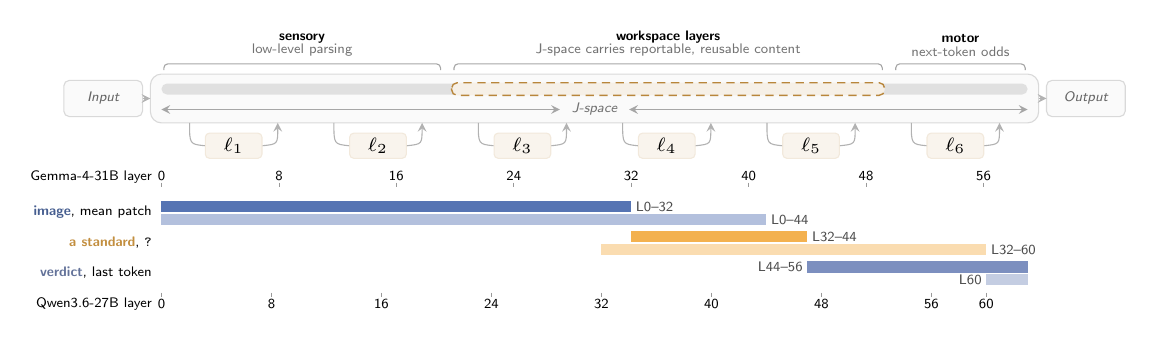
\begin{tikzpicture}
  \begin{scope}[font=\sffamily]
  \node[font=\tiny\sffamily, align=center, anchor=south, inner sep=1pt] at (4.537,-5.090) {\textbf{sensory}\\[-1pt]{\color{black!55}low-level parsing}};
  \draw[black!35, line width=.4pt, rounded corners=1.5pt] (2.780,-5.220) -- (2.780,-5.140) -- (6.295,-5.140) -- (6.295,-5.220);
  \node[font=\tiny\sffamily, align=center, anchor=south, inner sep=1pt] at (9.185,-5.090) {\textbf{workspace layers}\\[-1pt]{\color{black!55}J-space carries reportable, reusable content}};
  \draw[black!35, line width=.4pt, rounded corners=1.5pt] (6.465,-5.220) -- (6.465,-5.140) -- (11.905,-5.140) -- (11.905,-5.220);
  \node[font=\tiny\sffamily, align=center, anchor=south, inner sep=1pt] at (12.898,-5.090) {\textbf{motor}\\[-1pt]{\color{black!55}next-token odds}};
  \draw[black!35, line width=.4pt, rounded corners=1.5pt] (12.075,-5.220) -- (12.075,-5.140) -- (13.720,-5.140) -- (13.720,-5.220);
  \draw[black!15, fill=black!2, rounded corners=4pt] (2.61,-5.270) rectangle (13.89,-5.890);
  \fill[black!12, rounded corners=2pt] (2.75,-5.390) rectangle (13.75,-5.530);
  \draw[cworkspace, fill=cworkspace!12, densely dashed, line width=.5pt, rounded corners=2pt] (6.435,-5.380) rectangle (11.935,-5.540);
  \draw[black!35, <->, >=stealth, line width=.4pt] (2.75,-5.720) -- (7.810,-5.720);
  \draw[black!35, <->, >=stealth, line width=.4pt] (8.690,-5.720) -- (13.75,-5.720);
  \node[font=\tiny\sffamily\itshape, text=black!55, inner sep=0pt] at (8.250,-5.720) {J-space};
  \node[draw=black!15, fill=black!2, rounded corners=2pt, font=\tiny\sffamily\itshape, text=black!60, minimum width=1.0cm, minimum height=.46cm, inner sep=1pt] at (2.01,-5.580) {Input};
  \node[draw=black!15, fill=black!2, rounded corners=2pt, font=\tiny\sffamily\itshape, text=black!60, minimum width=1.0cm, minimum height=.46cm, inner sep=1pt] at (14.49,-5.580) {Output};
  \draw[black!30, ->, >=stealth, line width=.4pt] (2.51,-5.580) -- (2.61,-5.580);
  \draw[black!30, ->, >=stealth, line width=.4pt] (13.89,-5.580) -- (13.99,-5.580);
  \node[fill=cworkspace!9, draw=cworkspace!18, rounded corners=1.5pt, font=\scriptsize, minimum width=.72cm, minimum height=.32cm, inner sep=0pt] (l0) at (3.667,-6.180) {$\ell_1$};
  \draw[black!30, line width=.4pt] (3.107,-5.890) .. controls (3.107,-6.160) .. (l0.west);
  \draw[black!30, ->, >=stealth, line width=.4pt] (l0.east) .. controls (4.227,-6.160) .. (4.227,-5.890);
  \node[fill=cworkspace!9, draw=cworkspace!18, rounded corners=1.5pt, font=\scriptsize, minimum width=.72cm, minimum height=.32cm, inner sep=0pt] (l1) at (5.500,-6.180) {$\ell_2$};
  \draw[black!30, line width=.4pt] (4.940,-5.890) .. controls (4.940,-6.160) .. (l1.west);
  \draw[black!30, ->, >=stealth, line width=.4pt] (l1.east) .. controls (6.060,-6.160) .. (6.060,-5.890);
  \node[fill=cworkspace!9, draw=cworkspace!18, rounded corners=1.5pt, font=\scriptsize, minimum width=.72cm, minimum height=.32cm, inner sep=0pt] (l2) at (7.334,-6.180) {$\ell_3$};
  \draw[black!30, line width=.4pt] (6.774,-5.890) .. controls (6.774,-6.160) .. (l2.west);
  \draw[black!30, ->, >=stealth, line width=.4pt] (l2.east) .. controls (7.894,-6.160) .. (7.894,-5.890);
  \node[fill=cworkspace!9, draw=cworkspace!18, rounded corners=1.5pt, font=\scriptsize, minimum width=.72cm, minimum height=.32cm, inner sep=0pt] (l3) at (9.167,-6.180) {$\ell_4$};
  \draw[black!30, line width=.4pt] (8.607,-5.890) .. controls (8.607,-6.160) .. (l3.west);
  \draw[black!30, ->, >=stealth, line width=.4pt] (l3.east) .. controls (9.727,-6.160) .. (9.727,-5.890);
  \node[fill=cworkspace!9, draw=cworkspace!18, rounded corners=1.5pt, font=\scriptsize, minimum width=.72cm, minimum height=.32cm, inner sep=0pt] (l4) at (11.000,-6.180) {$\ell_5$};
  \draw[black!30, line width=.4pt] (10.440,-5.890) .. controls (10.440,-6.160) .. (l4.west);
  \draw[black!30, ->, >=stealth, line width=.4pt] (l4.east) .. controls (11.560,-6.160) .. (11.560,-5.890);
  \node[fill=cworkspace!9, draw=cworkspace!18, rounded corners=1.5pt, font=\scriptsize, minimum width=.72cm, minimum height=.32cm, inner sep=0pt] (l5) at (12.833,-6.180) {$\ell_6$};
  \draw[black!30, line width=.4pt] (12.273,-5.890) .. controls (12.273,-6.160) .. (l5.west);
  \draw[black!30, ->, >=stealth, line width=.4pt] (l5.east) .. controls (13.393,-6.160) .. (13.393,-5.890);
  % Dark bars are Gemma-4-31B, on the top scale. Light bars are Qwen3.6-27B, on the bottom scale.
  \node[anchor=east, font=\tiny\sffamily, inner sep=1pt] at (2.67,-6.580) {Gemma-4-31B layer};
  \draw[black!40, line width=.3pt] (2.750,-6.650) -- (2.750,-6.710);
  \node[font=\tiny\sffamily, inner sep=0pt] at (2.750,-6.570) {0};
  \draw[black!40, line width=.3pt] (4.242,-6.650) -- (4.242,-6.710);
  \node[font=\tiny\sffamily, inner sep=0pt] at (4.242,-6.570) {8};
  \draw[black!40, line width=.3pt] (5.733,-6.650) -- (5.733,-6.710);
  \node[font=\tiny\sffamily, inner sep=0pt] at (5.733,-6.570) {16};
  \draw[black!40, line width=.3pt] (7.225,-6.650) -- (7.225,-6.710);
  \node[font=\tiny\sffamily, inner sep=0pt] at (7.225,-6.570) {24};
  \draw[black!40, line width=.3pt] (8.716,-6.650) -- (8.716,-6.710);
  \node[font=\tiny\sffamily, inner sep=0pt] at (8.716,-6.570) {32};
  \draw[black!40, line width=.3pt] (10.208,-6.650) -- (10.208,-6.710);
  \node[font=\tiny\sffamily, inner sep=0pt] at (10.208,-6.570) {40};
  \draw[black!40, line width=.3pt] (11.699,-6.650) -- (11.699,-6.710);
  \node[font=\tiny\sffamily, inner sep=0pt] at (11.699,-6.570) {48};
  \draw[black!40, line width=.3pt] (13.191,-6.650) -- (13.191,-6.710);
  \node[font=\tiny\sffamily, inner sep=0pt] at (13.191,-6.570) {56};
  \node[anchor=east, font=\tiny\sffamily, inner sep=1pt, align=right] at (2.67,-7.020) {\textbf{\color{cscene!80!black}image}, mean patch};
  \fill[cscene] (2.750,-6.880) rectangle (8.716,-7.020);
  \node[anchor=west, font=\tiny\sffamily, text=black!70, inner sep=1.5pt] at (8.716,-6.950) {L0--32};
  \fill[cscene!45] (2.750,-7.045) rectangle (10.433,-7.185);
  \node[anchor=west, font=\tiny\sffamily, text=black!70, inner sep=1.5pt] at (10.433,-7.115) {L0--44};
  \node[anchor=east, font=\tiny\sffamily, inner sep=1pt, align=right] at (2.67,-7.405) {\textbf{\color{cstandard!80!black}a standard}, \texttt{?}};
  \fill[cstandard] (8.716,-7.265) rectangle (10.953,-7.405);
  \node[anchor=west, font=\tiny\sffamily, text=black!70, inner sep=1.5pt] at (10.953,-7.335) {L32--44};
  \fill[cstandard!45] (8.337,-7.430) rectangle (13.226,-7.570);
  \node[anchor=west, font=\tiny\sffamily, text=black!70, inner sep=1.5pt] at (13.226,-7.500) {L32--60};
  \node[anchor=east, font=\tiny\sffamily, inner sep=1pt, align=right] at (2.67,-7.790) {\textbf{\color{cverdict!80!black}verdict}, last token};
  \fill[cverdict] (10.953,-7.650) rectangle (13.750,-7.790);
  \node[anchor=east, font=\tiny\sffamily, text=black!70, inner sep=1.5pt] at (10.953,-7.720) {L44--56};
  \fill[cverdict!45] (13.226,-7.815) rectangle (13.750,-7.955);
  \node[anchor=east, font=\tiny\sffamily, text=black!70, inner sep=1.5pt] at (13.226,-7.885) {L60};
  \node[anchor=east, font=\tiny\sffamily, inner sep=1pt] at (2.67,-8.185) {Qwen3.6-27B layer};
  \draw[black!40, line width=.3pt] (2.750,-8.045) -- (2.750,-8.105);
  \node[font=\tiny\sffamily, inner sep=0pt] at (2.750,-8.185) {0};
  \draw[black!40, line width=.3pt] (4.147,-8.045) -- (4.147,-8.105);
  \node[font=\tiny\sffamily, inner sep=0pt] at (4.147,-8.185) {8};
  \draw[black!40, line width=.3pt] (5.544,-8.045) -- (5.544,-8.105);
  \node[font=\tiny\sffamily, inner sep=0pt] at (5.544,-8.185) {16};
  \draw[black!40, line width=.3pt] (6.940,-8.045) -- (6.940,-8.105);
  \node[font=\tiny\sffamily, inner sep=0pt] at (6.940,-8.185) {24};
  \draw[black!40, line width=.3pt] (8.337,-8.045) -- (8.337,-8.105);
  \node[font=\tiny\sffamily, inner sep=0pt] at (8.337,-8.185) {32};
  \draw[black!40, line width=.3pt] (9.734,-8.045) -- (9.734,-8.105);
  \node[font=\tiny\sffamily, inner sep=0pt] at (9.734,-8.185) {40};
  \draw[black!40, line width=.3pt] (11.131,-8.045) -- (11.131,-8.105);
  \node[font=\tiny\sffamily, inner sep=0pt] at (11.131,-8.185) {48};
  \draw[black!40, line width=.3pt] (12.528,-8.045) -- (12.528,-8.105);
  \node[font=\tiny\sffamily, inner sep=0pt] at (12.528,-8.185) {56};
  \draw[black!40, line width=.3pt] (13.226,-8.045) -- (13.226,-8.105);
  \node[font=\tiny\sffamily, inner sep=0pt] at (13.226,-8.185) {60};
  \end{scope}
\end{tikzpicture}
